\section{Operational constraints identify reversal}

E2 assigns budget, rotation, contract and dominant-crop-bound interventions while holding the ranking and scenario law fixed (Fig.~\ref{fig:operations}). The base allocation assigns corn share \EtwoBaseCorn{}. Each treated cell instead assigns a soybean majority: contract or rotation interventions produce corn and soybean shares \EtwoForcedCorn{} and \EtwoForcedSoy{}, while the tighter budget produces \EtwoBudgetCorn{} and \EtwoBudgetSoy{}. Possible, universal and selected reversal coincide in every treated cell, including the bound anchor.

All \EtwoPassedIntervals{} of \EtwoIntervals{} registered family-wise intervals meet their precision targets at \EtwoReplications{} replications per cell. The optimal-face classifications rule out selection dependence, and the local KKT audit shows that the loss-CVaR term is inactive in these cells. Because the intervention is assigned within a closed simulation, E2 identifies an operational displacement mechanism in its declared domain. It does not estimate how often that mechanism operates in agriculture.

The evidence rule is experiment-level rather than contrast-level. E1, E3, E4 and E5 each reach their registered ceiling without meeting every primary precision criterion. Passing rows inside those experiments do not rescue the experiment. E1 is reported in Supplementary Fig.~S1, E3 in Supplementary Fig.~S2, and E4/E5 in Supplementary Fig.~S3. All \RegisteredInfeasible{} registered infeasible rows remain in the evidence ledger; no feasible-only subset enters a positive claim.

\begin{figure}[t]
\centering
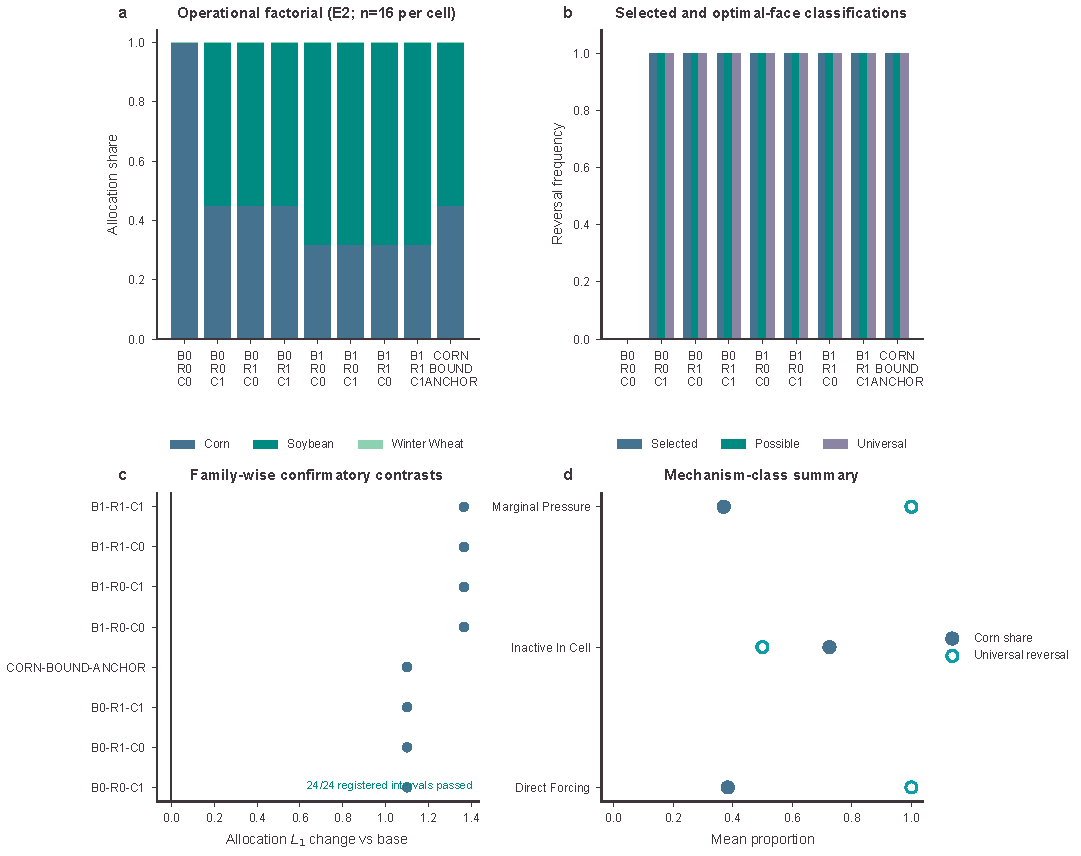
\includegraphics[width=\textwidth]{../figures/stage_ii/main/Figure4.pdf}
\caption{\textbf{Operational interventions identify reversal in E2.} The E2-only display reports the factorial allocation, selected and optimal-face classifications, family-wise contrasts and mechanism-class summaries. Each cell has $n=\EtwoReplications{}$ and all \EtwoPassedIntervals{}/\EtwoIntervals{} intervals meet the pre-specified precision criterion.}
\label{fig:operations}
\end{figure}
